\documentclass[a4paper, 12pt]{article}

\usepackage[left=2cm,right=2cm,
    top=2cm,bottom=2cm,bindingoffset=0cm]{geometry}

\usepackage[T2A]{fontenc}
\usepackage[utf8]{inputenc}
\usepackage{color}
\usepackage{graphicx}
\usepackage{caption}
\usepackage{subcaption}
\usepackage{tikz}
\usepackage[english, russian]{babel}
\usepackage{ gensymb }
\usepackage{booktabs}
\usepackage{amsmath,amsfonts,amssymb,amsthm,mathtools}
\usepackage{lscape}
\usepackage{listings}

\begin{document}


\begin{center}
\textbf{Треугольные конечные элементы высшего порядка.}
\end{center}
\begin{center}
\textbf{\textit{Задание}}
\end{center}

\begin{enumerate}
    \item Определить функции формы для квадратичного треугольного элемента. Записать общую процедуру вывода и объяснить.
    \item Вычислить \(\displaystyle \frac{\partial N_i}{\partial x}, \frac{\partial N_i}{\partial y}\) в произвольной точке $k = 1 \dots 6 \neq i$ для квадратичного изопараметрического треугольного элемента (см. рисунок), где $i = 1 \dots 6$ – номер варианта по журналу.
    \item Вычислить численно интеграл \(\displaystyle \iint \limits_S \left ( \frac{\partial N_i}{\partial x} \cdot \frac{\partial N_i}{\partial y} \right ) dS\) по площади треугольного элемента (см. рисунок). Проверить ответ, применив формулу 
    \[\displaystyle \int \limits_{S^{(e)}} L_1^{\alpha} L_2^{\beta} L_3^{\gamma} dS = \frac{\alpha! \beta! \gamma!}{(\alpha + \beta + \gamma + 2)!} \cdot 2S^{(e)}\].
\end{enumerate}

\begin{center}
    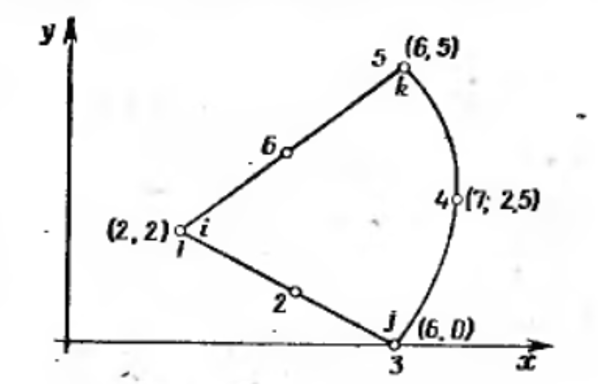
\includegraphics{zad.png}
\end{center}


\begin{center}
    \textbf{\textit{Решение}}
\end{center}

\begin{enumerate}
    \item Функции формы определяются через $L$ координаты. Так как
    функция формы $N_i$ в узле $i$ должна равняться 1, а в остальных 0, то её
    можно определить как произведение функций прямых, проходящих
    через все узлы, кроме $i$-го:
    \[N_{\beta} = \prod_{\delta=1}^n \frac{F_{\delta}}{F_{\delta} |_{L_1,L_2,L_3}},\ F_{\delta} - \text{ пробные функции},\]

    где n -- степень конечного элемента.

    \begin{center}
        \begin{tabular}{cc}
            \begin{tikzpicture}
                    \draw[->] (-0.2,0) -- (5,0) node[right] {$x$};
                    \draw[->] (0,-0.2) -- (0,3) node[above] {$y$};
                    \draw[blue, thick] (1,0.5) -- (4,1) -- (2,2.5) -- cycle;
                {\footnotesize
                    \node at (1.5,0.55) [below left] {$1$};
                    \node at (4,1) [above right] {$3$};
                    \node at (2,2.5) [above] {$5$};
                \node at (2.3, 0.72)[below] {$2$};
                \node at (1.6, 1.7)[left] {$6$};
                \node at (2.75, 1.95)[above right] {$4$};
                }
                \fill[blue] (1, 0.5) circle (1pt);
                \fill[blue] (4,1) circle (1pt);
                \fill[blue] (2,2.5) circle (1pt);
                \fill[blue] (2.3, 0.72) circle (1pt);
                \fill[blue] (1.6, 1.7) circle (1pt);
                \fill[blue] (2.75, 1.95) circle (1pt);
        
                \draw[->][thin, teal] (2.3, 0.72) -- (2.21,1.25) node[right] {\footnotesize $L_3$};
                \draw[->][thin, red] (1.6, 1.7) -- (2.15,1.35) node[above] {\footnotesize $L_2$};
                \draw[->][thin] (2.75, 1.95) -- (2.5,1.6) node[above] {\footnotesize $L_1$};
            \end{tikzpicture}
            & 

            \begin{tikzpicture}
                    \draw[blue, thick] (1,0.5) -- (4,1) -- (2,2.5) -- cycle;
                    {\footnotesize
                        \node at (1.5,0.55) [below left] {$1$};
                    \node at (1.9, 0.1)[below left] {$(1,0,0)$};
                    \node at (4,1) [right] {$3$};
                    \node at (4.5, 1)[right] {$(0,1,0)$};
                        \node at (2,2.5) [above] {$5$};
                    \node at (2.3, 0.72)[below] {$2$};
                    \node at (2.7, 0.35)[below] {$\footnotesize(\frac{1}{2},\frac{1}{2},0)$};
                    \node at (1.4, 1.3)[above] {$6$};
                    \node at (2.85, 1.85)[above right] {$4$};
                    }
                    \fill[blue] (1, 0.5) circle (1pt);
                    \fill[blue] (4,1) circle (1pt);
                    \fill[blue] (2,2.5) circle (1pt);
                    \fill[blue] (2.3, 0.72) circle (1pt);
                    \fill[blue] (1.4, 1.3) circle (1pt);
                    \fill[blue] (2.85, 1.85) circle (1pt);
                    
                    \draw[thin, red] (0.5,-0.5) -- (2.5, 3.5) node[above right] {\footnotesize $L_2 - 0$};
                    \draw[thin, red] (1.725, -0.5) -- (3.35, 2.89) node[right] {\footnotesize $L_2 - \frac{1}{2}$};
                    \draw[thin, red] (3.25,-0.5) -- (5.25, 3.5) node[right] {\footnotesize $L_2 - 1$};
                    
                    \draw[thin] (5,0.25) -- (1, 3.25) node[above] {\footnotesize $L_1 - 0$};
                    \draw[thin] (4,-1.35) -- (0, 1.15) node[below left] {\footnotesize $L_1 - 1$};
                    \draw[thin] (4.4, -0.63) -- (0.8, 1.68) node[above left] {\footnotesize $L_1 -  \frac{1}{2}$};
                \end{tikzpicture}
                \\
            \end{tabular}
        \end{center}

Функции формы:
\[N_1 = \frac{L_1 \left(L_1 - \displaystyle\frac{1}{2}\right)}{1 \left(1 - \displaystyle\frac{1}{2}\right)} = L_1 (2L_1 - 1)\]
\[N_2 = \frac{L_2L_1}{\displaystyle\frac{1}{2} \cdot \frac{1}{2}} = 4L_1L_2\]
\[N_3 = \frac{L_2 \left(L_2 - \displaystyle\frac{1}{2}\right)}{1 \left(1 - \displaystyle\frac{1}{2}\right)} = L_2 (2L_2 - 1)\]
\[N_4 = 4L_2L_3\]
\[N_5 = L_3(2L_3 - 1)\]
\[N_6 = 4L_1L_3\]

\item Вычислим производные от функций форм

\begin{center}
	\begin{tabular}{c|c}
		Точка & Координаты точки \\
		\hline
		1 & 2 \qquad 2 \\
		\hline
        2 & 4 \qquad 1 \\
		\hline
		3 & 6 \qquad 0 \\
        \hline
		4 & 7 \quad \  2.5 \\
		\hline
		5 & 6 \qquad 5 \\
        \hline
        6 & 4 \quad \  3.5 \\
		\hline
	\end{tabular}
\end{center}

\[
    \begin{cases}
		x = \sum \limits_{k=1}^6 x_k N_k = 2L_1 (2L_1 - 1) + 4 \cdot 4L_1L_2 + 6 L_2 (2L_2 - 1) + 7 \cdot 4L_2L_3 + 6 \cdot L_3(2L_3 - 1) + 4 \cdot 4L_1L_3\\
		y= \sum \limits_{k=1}^6 y_k N_k = 2L_1 (2L_1 - 1) + 1 \cdot 4L_1L_2 + 2.5 \cdot 4L_2L_3 + 5 \cdot L_3(2L_3 - 1) + 3.5 \cdot 4L_1L_3
	\end{cases}
\]
\[
    \begin{cases}
		x = 2L_1 (2L_1 - 1) + 16L_1L_2 + 6 L_2 (2L_2 - 1) + 28L_2L_3 + 6 \cdot L_3(2L_3 - 1) + 16L_1L_3\\
		y= 2L_1 (2L_1 - 1) + 4L_1L_2 + 10L_2L_3 + 5 L_3(2L_3 - 1) + 14L_1L_3
	\end{cases}
\]
\[
    L_3 = 1 - L_1 - L_2
\]
Якобиан:
\[
    J = \begin{bmatrix}
        \frac{\partial x}{\partial L_1} & \frac{\partial y}{\partial L_1} \\ 
        \frac{\partial x}{\partial L_2} & \frac{\partial y}{\partial L_2} 
        \end{bmatrix}
\]
\[
	\begin{bmatrix}
		\frac{\partial N_{\beta}}{\partial x} \\ \frac{\partial N_{\beta}}{\partial y}
	\end{bmatrix} = J^{-1} \cdot \begin{bmatrix}
	\frac{\partial N_{\beta}}{\partial L_1} \\ \frac{\partial N_{\beta}}{\partial L_2}
	\end{bmatrix}
\]
\[
\begin{cases}
    \frac{\partial x}{\partial L_1} = -4L_2 + 4,\\
    \frac{\partial y}{\partial L_1} = -3,\\
    \frac{\partial x}{\partial L_2} = -4L_1 -8L_2 + 4,\\
    \frac{\partial y}{\partial L_2} = -5
\end{cases}
\]
\[
    J = \begin{bmatrix}
        -4L_2 - 4 & -3 \\ 
        -4L_1 -8L_2 + 4 & -5 
        \end{bmatrix}
    \Rightarrow
    J^{-1} = \begin{bmatrix}
        \frac{5}{12L_1+4L_2-32} & -\frac{3}{12L_1+4L_2-32} \\
        \frac{-L_1-2L_2+1}{3L_1+L_2-8} & \frac{L_2+1}{3L_1+L_2-8}
    \end{bmatrix}
\]
\[
    \begin{bmatrix}
        \frac{\partial N_{3}}{\partial L_1} \\ \frac{\partial N_{3}}{\partial L_2}
        \end{bmatrix} =
        \begin{bmatrix}
            0 \\ 4L_2 - 1
        \end{bmatrix}
\]
\[
	\begin{bmatrix}
		\frac{\partial N_{3}}{\partial x} \\ \frac{\partial N_{3}}{\partial y}
	\end{bmatrix} = \begin{bmatrix}
        \frac{5}{12L_1+4L_2-32} & -\frac{3}{12L_1+4L_2-32} \\
        \frac{-L_1-2L_2+1}{3L_1+L_2-8} & \frac{L_2+1}{3L_1+L_2-8}
    \end{bmatrix} \cdot
    \begin{bmatrix}
        0 \\ 4L_2 - 1
    \end{bmatrix} =
    \begin{bmatrix}
        \frac{-12L_2 + 3}{12L_1+4L_2-32} \\ \frac{(L_2+1)(4L_2 - 1)}{3L_1+L_2-8}
    \end{bmatrix}
\]

Выберем узел \(i=3\):
\[
    L_1 = 0,\ L_2 = 1
\]
\[
    \begin{bmatrix}
        \frac{\partial N_{3}}{\partial x} \\ \frac{\partial N_{3}}{\partial y}
        \end{bmatrix} =
        \begin{bmatrix}
            \frac{9}{28} \\ -\frac{6}{7}
        \end{bmatrix}
\]
\item \(\displaystyle \iint \limits_S \left ( \frac{\partial N_3}{\partial x} \cdot \frac{\partial N_3}{\partial y} \right ) dS = 
\int \limits_0^1 \int \limits_0^{1-L_1} \left ( \frac{\partial N_3}{\partial x} \cdot \frac{\partial N_3}{\partial y} \right ) \cdot |J| dL_2 dL_1\)

\[
    \frac{\partial N_3}{\partial x} \cdot \frac{\partial N_3}{\partial y} = 
    \frac{-12L_2 + 3}{12L_1+4L_2-32} \cdot \frac{(L_2+1)(4L_2 - 1)}{3L_1+L_2-8}
\]
Для численного интегрирования будем использовать схему третьего порядка точности:
\begin{center}
    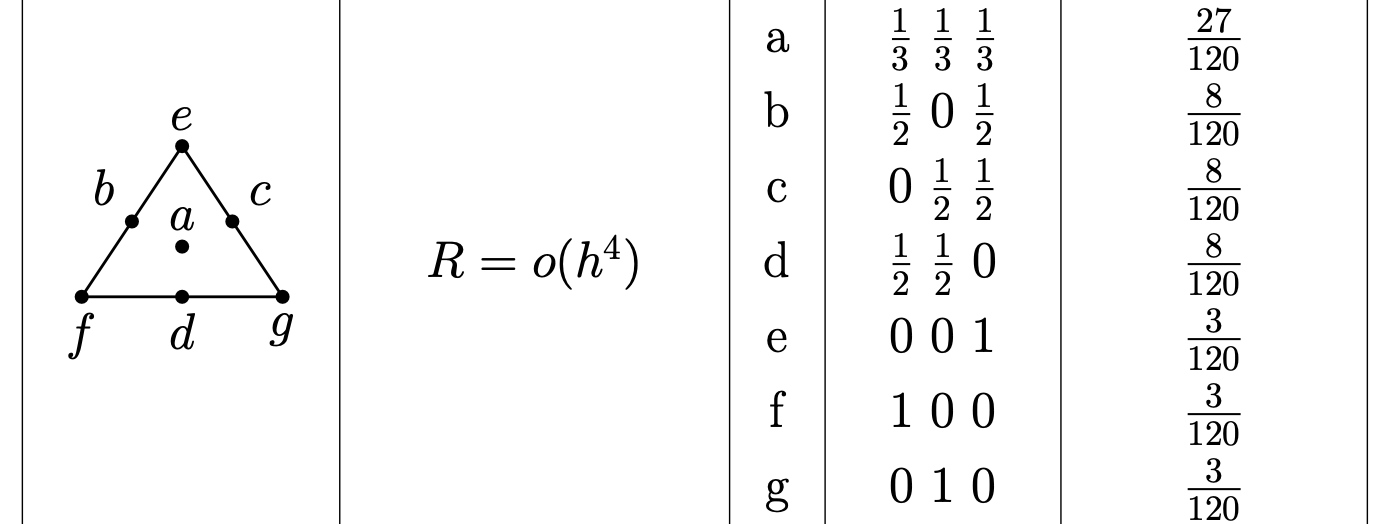
\includegraphics[scale=0.3]{table.png}
\end{center}
\[
    Z = \int \limits_0^1 \int \limits_0^{1-L_1} \left ( \frac{\partial N_3}{\partial x} \cdot \frac{\partial N_3}{\partial y} \right ) \cdot |J| dL_2 dL_1 =
    \sum \limits_{i=1}^3 W_i g_i (L_1, L_2, L_3)
\]
\[
    g_i (L_1, L_2, L_3) = \frac{\partial N_3}{\partial x} \cdot \frac{\partial N_3}{\partial y} \cdot |J| =
    \frac{(12L_2-3)(-16L_2^2+20L_2-4)}{4L_2 + 8 + 12L_1}
\]
\[
    \begin{cases}
        g_1 = \frac{(4-3)(-16/9+20/3-4)}{4/3 + 8 + 4} = \frac{1}{15},\\
        g_2 = \frac{(-3)(-4)}{8 + 6} = \frac{6}{7},\\
        g_3 = \frac{(6-3)(-4+10-4)}{2 + 8} = \frac{3}{5},\\
        g_4 = \frac{(6-3)(-4+10-4)}{2 + 8 + 6} = \frac{3}{8},\\
        g_5 = \frac{(-3)(-4)}{8} = \frac{3}{2},\\
        g_6 = \frac{(-3)(-4)}{8 + 12} = \frac{3}{5},\\
        g_7 = \frac{(12-3)(-16+20-4)}{4 + 8} = 0
    \end{cases}
\]
\[
    Z = \frac{27}{120} \cdot \frac{1}{15} + \frac{8}{120} \cdot 
    \left(\frac{6}{7} + \frac{3}{5} + \frac{3}{8}\right) +
    \frac{3}{120} \cdot 
    \left(\frac{3}{2} + \frac{3}{5} + 0\right) = \frac{171}{560} \approx 0.1896
\]


\end{enumerate}
\end{document}